\newpage % Rozdziały zaczynamy od nowej strony.
\section{Rozwiązanie}
\subsection{Przegląd rozwiązań}

\begin{figure}[ht!]
    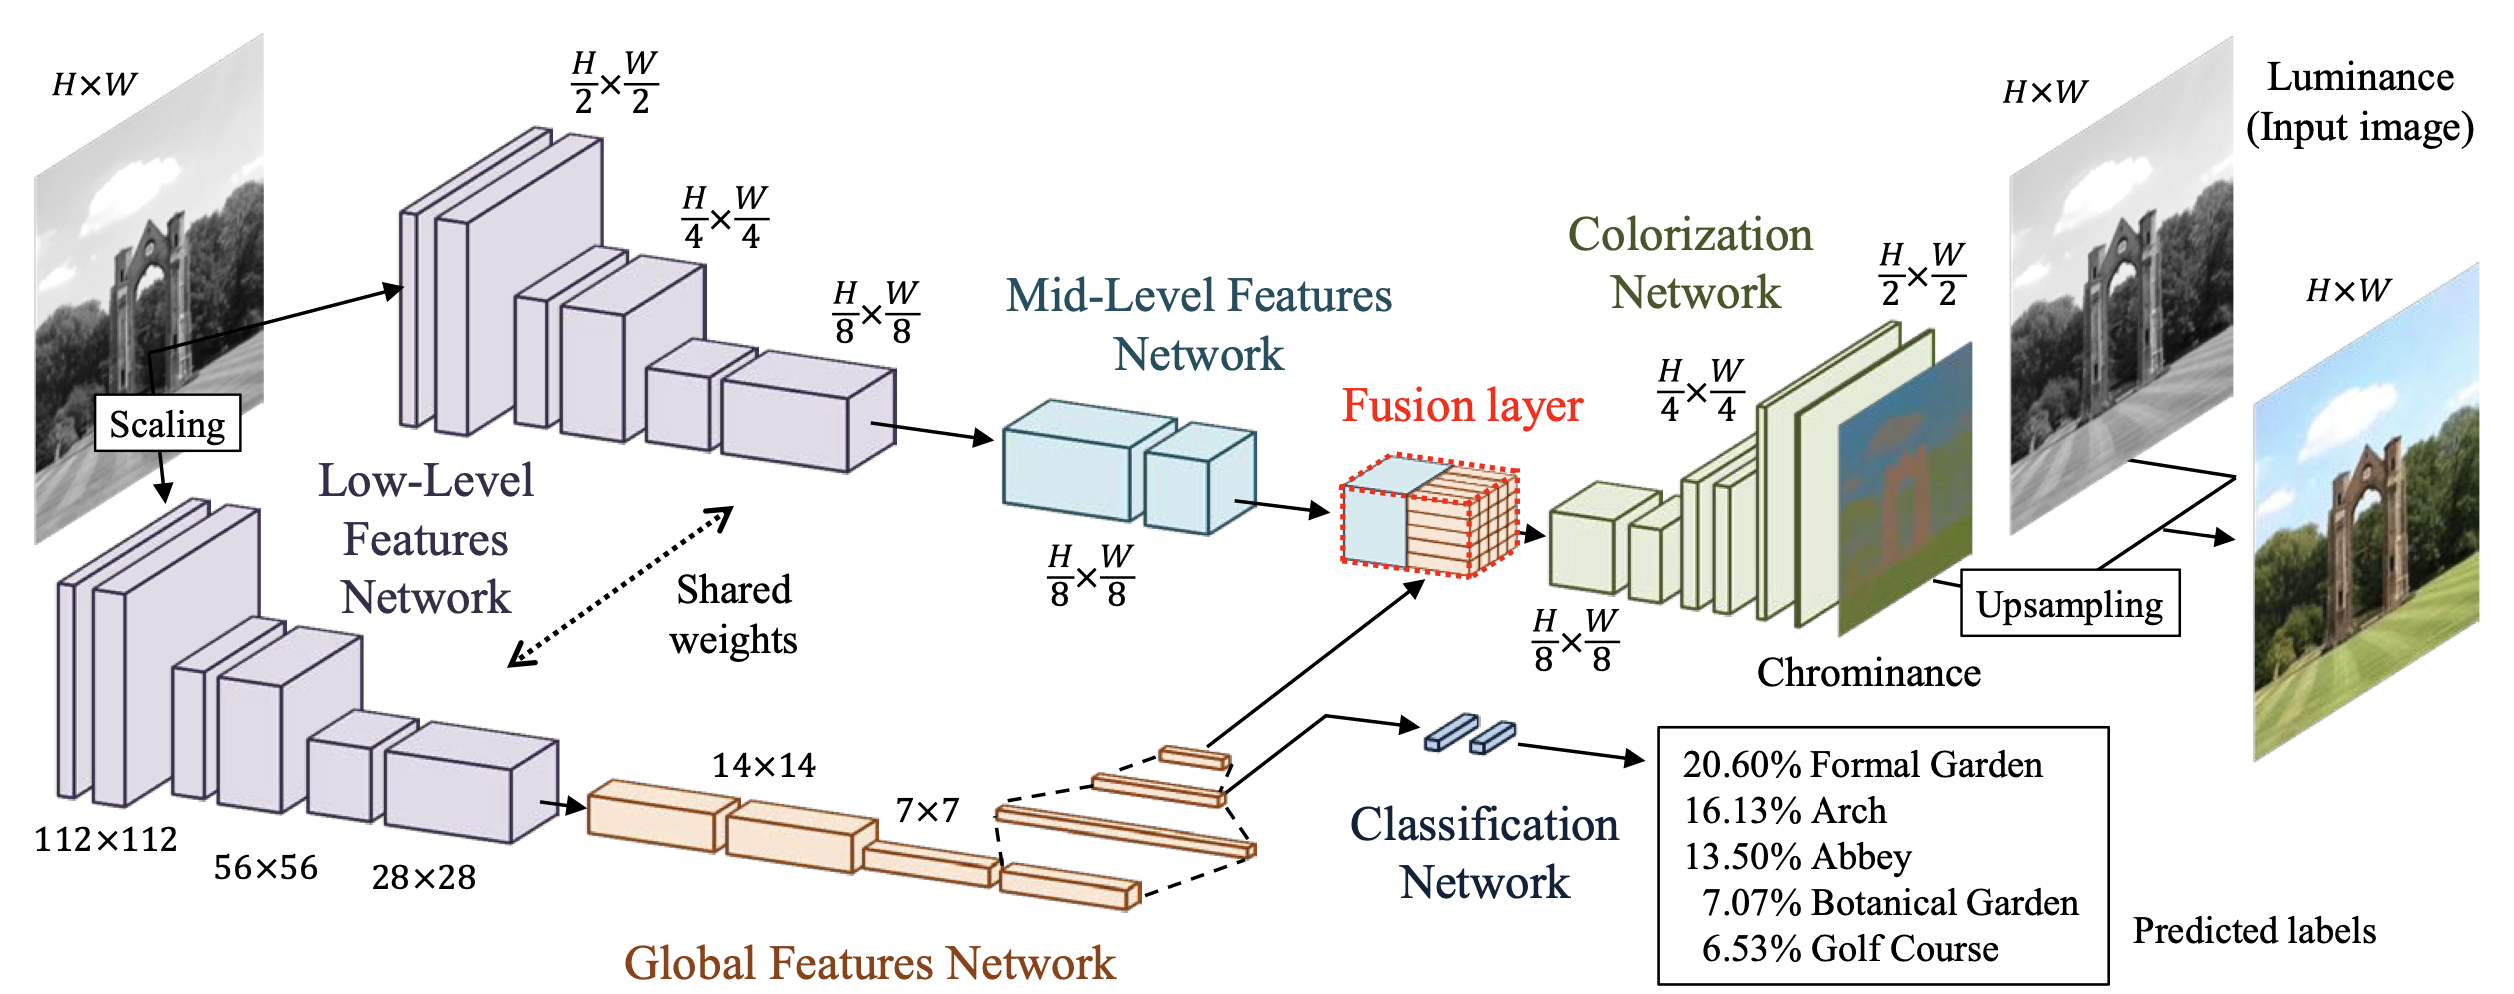
\includegraphics[width=\textwidth]{global-local-features.png}
    \caption{Let there be Color!: Joint End-to-end Learning of Global and Local Image Priors for Automatic Image Colorization with Simultaneous Classification 2016 \cite{iizuka2016let}.}
    \label{fig:parrarel-arch}
\end{figure}

Współcześnie do zadań wizji komputerowej używa się głębokich sieci neuronowych z uwagi na ich duże zdolności generalizacji skomplikowanych przestrzeni. Celem każdej architektury jest odpowiednia ekstrakcja cech w sposób łatwo ekstrahowalny. Architektury różnią się zatem sposobem generalizacji, a dokładniej ułożeniem warstw i ich parametrów. W ramach przeglądu literatury pochylono się nad różnymi metodami łączenia zadania segmentacji i klasyfikacji, ponieważ zadanie postawione w pracy, co do wiedzy autora, nie zostało wcześniej rozwiązane podobnymi metodami.

Pierwszy artykuł ,,Let there be Color!: Joint End-to-end Learning of Global and Local Image Priors for Automatic Image Colorization with Simultaneous Classification 2016 \cite{iizuka2016let}'' rozwiązuje problem kolorowania obrazków jednak, przekształcony może być użyty w pracy. Tego można dokonać odrzucając ostatnią warstwę konkatenacji w części segmentacji (rys. \ref{fig:parrarel-arch}). Przedstawiona architektura symultanicznie ekstrahuję cechy globalne oraz średniego poziomu, które odpowiednio służą klasyfikacji oraz segmentacji.

\begin{figure}[ht!]
    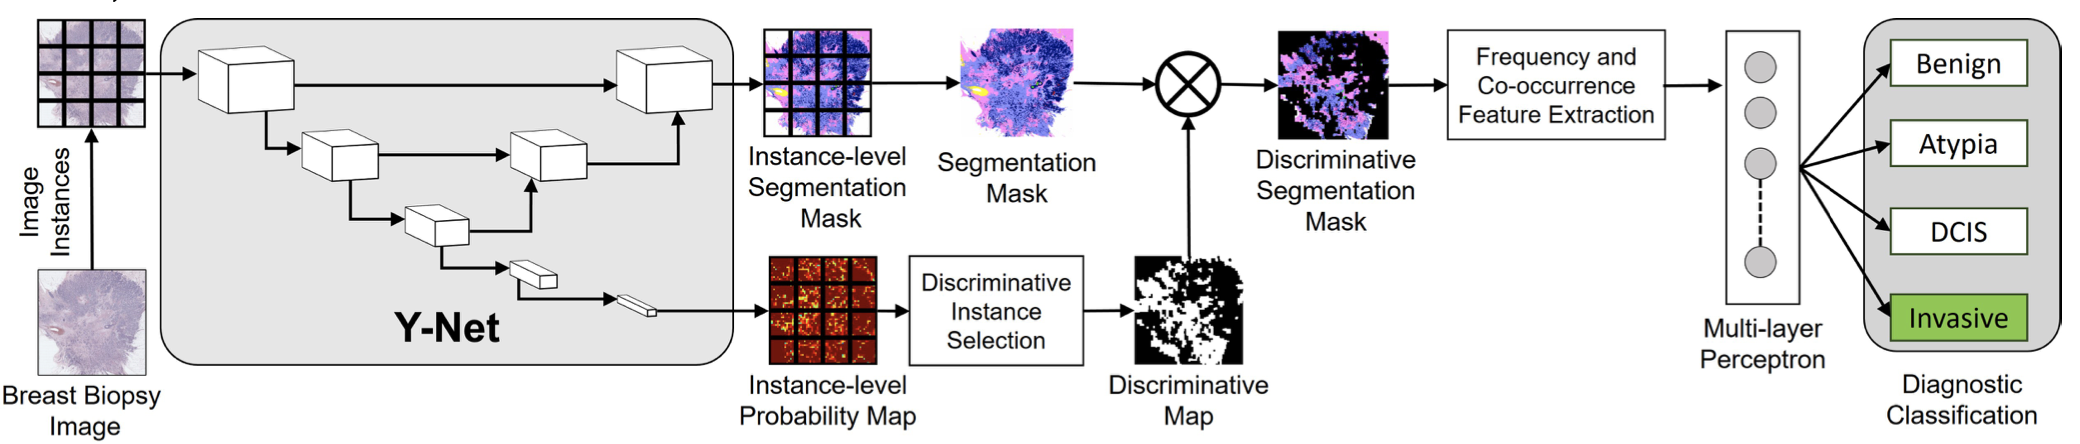
\includegraphics[width=\textwidth]{y-net.png}
    \caption{Y-Net: Joint Segmentation and Classification for Diagnosis of Breast Biopsy Images 2018 \cite{mehta2018net}.}
    \label{fig:y-net}
\end{figure}

Kolejnym artykułem jest ,,Y-Net: Joint Segmentation and Classification for Diagnosis of Breast Biopsy Images 2018 \cite{mehta2018net}''. Jest to standardowa architektura segmentacji \texttt{U-Net} rozszerzona o gałąź klasyfikacyjną (rys. \ref{fig:y-net}). Rozwiązanie to jest na pewno ciekawe z punku widzenia modularności rozwiązania.

\subsection{Zarys rozwiązania problemu}
% * multitask Learning
% * jednozadaniowe
% * wielozadaniowe
W celu realizacji zadania zdecydowano się na architekturę (najbliższą Y-Netu) o wspólnym enkoderze i o osobnych głowach, służących do egzekwowania konkretnych zadań (rys. \ref{fig:cep_arch}). Decyzja podyktowana była względnie prostą implementacją rozszerzenia wielu modeli segmentacji semantycznej o dodatkową głowę klasyfikacyjną. Co więcej stwierdzono, że ograniczenie się tylko do jednego backbone'u jest niesłychanie korzystne, gdyż znacząco ogranicza ilość parametrów sieci, co bezpośrednio przekłada się m.in. na czas inferencji. Należy zwrócić uwagę na fakt, iż właściwie zdecydowana większość parametrów znajduje się własnie w enkoderze.

Mając na uwadze, że symultaniczne uczenie może negatywnie wpływać na jakość uczenia obu zadań, eksperymenty przeprowadzono etapowo. Pierwszym etapem było uczenie jednozadaniowe. Eksperymenty polegały na sprawdzeniu jakości segmentacji oraz klasyfikacji osobno. Wykorzystano do tego tę samą archtekturę, która używana była poźniej w drugim etapie. Mianowicie, mając dwie głowy każdorazowo zamrażano głowę nie biorącą udziału w uczeniu (rys. \ref{fig:arch-scene-seg}). Zapewnia to pewność posiadania tej samej architektury, a w szczególności rzetelne porównanie z etapem uczenia wielozadaniowego.

Drugim etapem było przeprowadzenie eksperymentów w uczeniu wielozadaniowym (rys. \ref{fig:arch-full}). Funkcja celu zdefiniowana była jako suma wartości funkcji celów dla obu zadań. W wyniku progpagacji wstecznej wagi aktualizowane były zgodnie z zagregowaną stratą.

Ostatecznie porównano jakość na przesztreni obu etapów.

\begin{figure}[ht!]
    \centering
    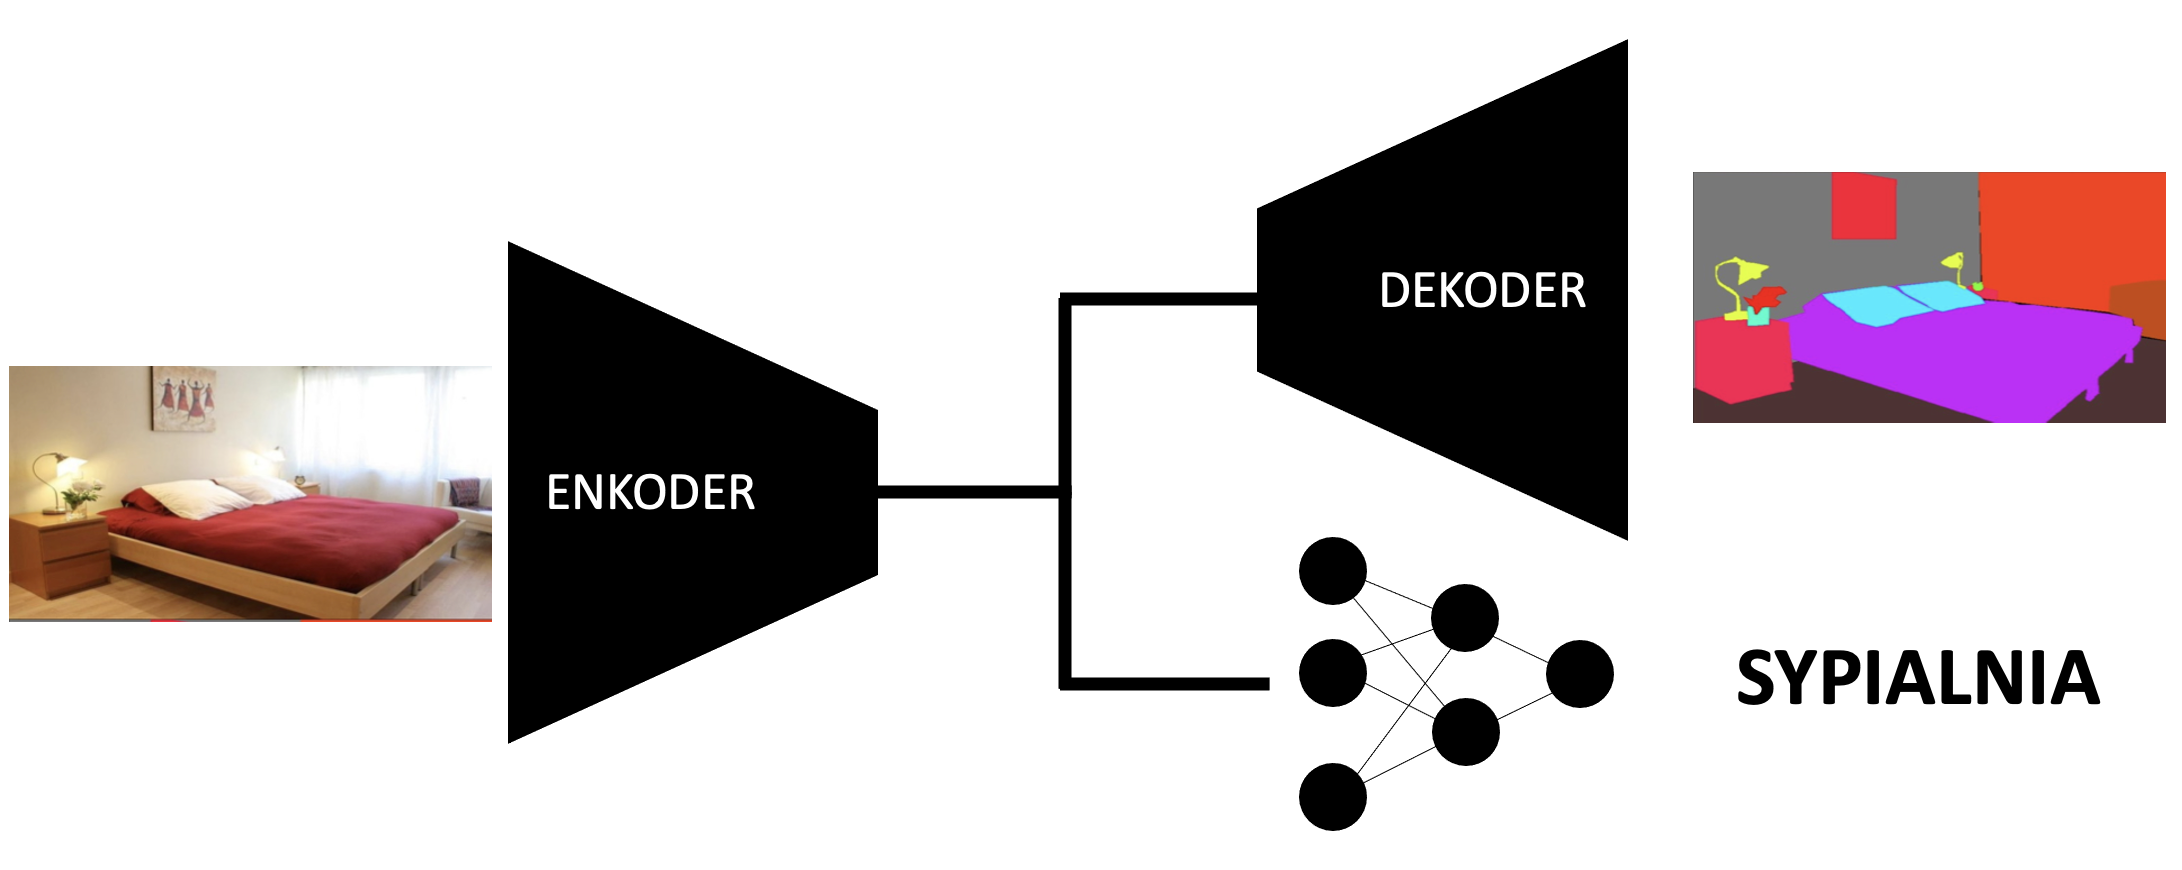
\includegraphics[width=0.75\textwidth]{cep_arch.png}
    \caption{Architektura sieci zastosowana w pracy inżynierskiej.}
    \label{fig:cep_arch}
\end{figure}

\begin{figure}[ht!]
    \centering
    \begin{subfigure}[b]{0.49\textwidth}
        \centering
        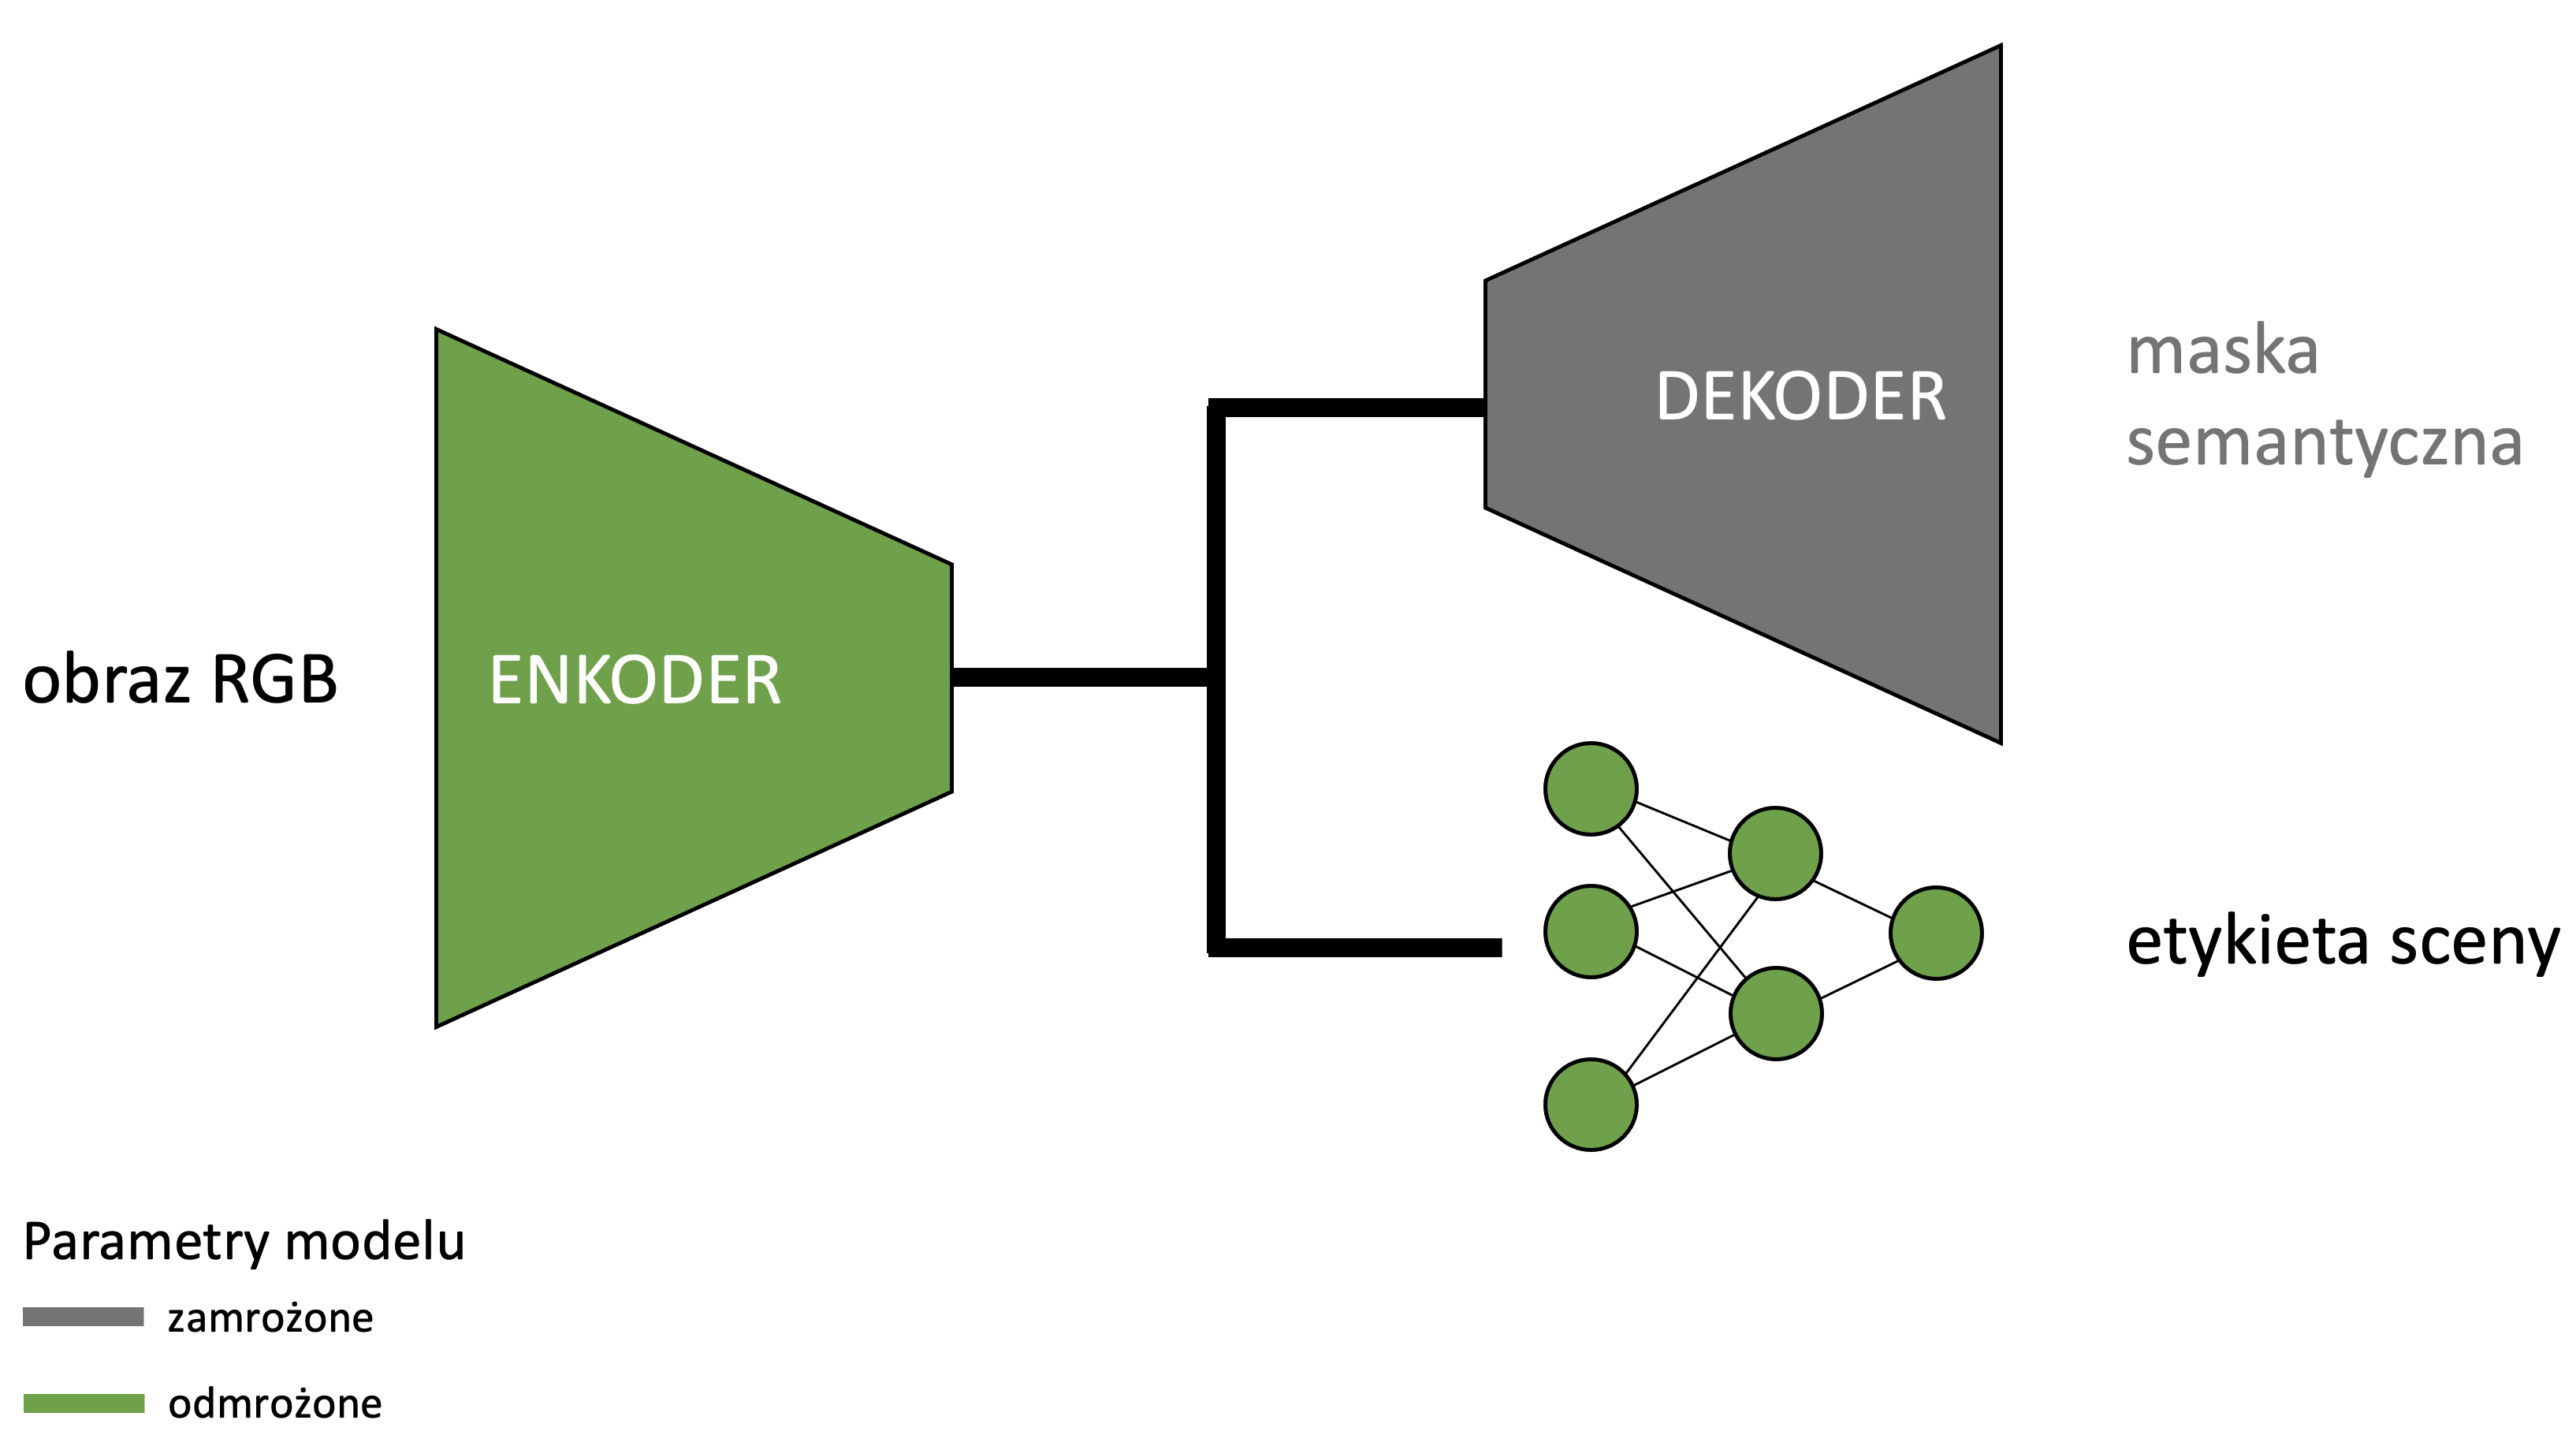
\includegraphics[width=\textwidth]{arch:scene.png}
        \caption{Architektura sieci wyłącznie w zadaniu klasyfikacji.}
    \end{subfigure}
    \hfill
    \begin{subfigure}[b]{0.49\textwidth}
        \centering
        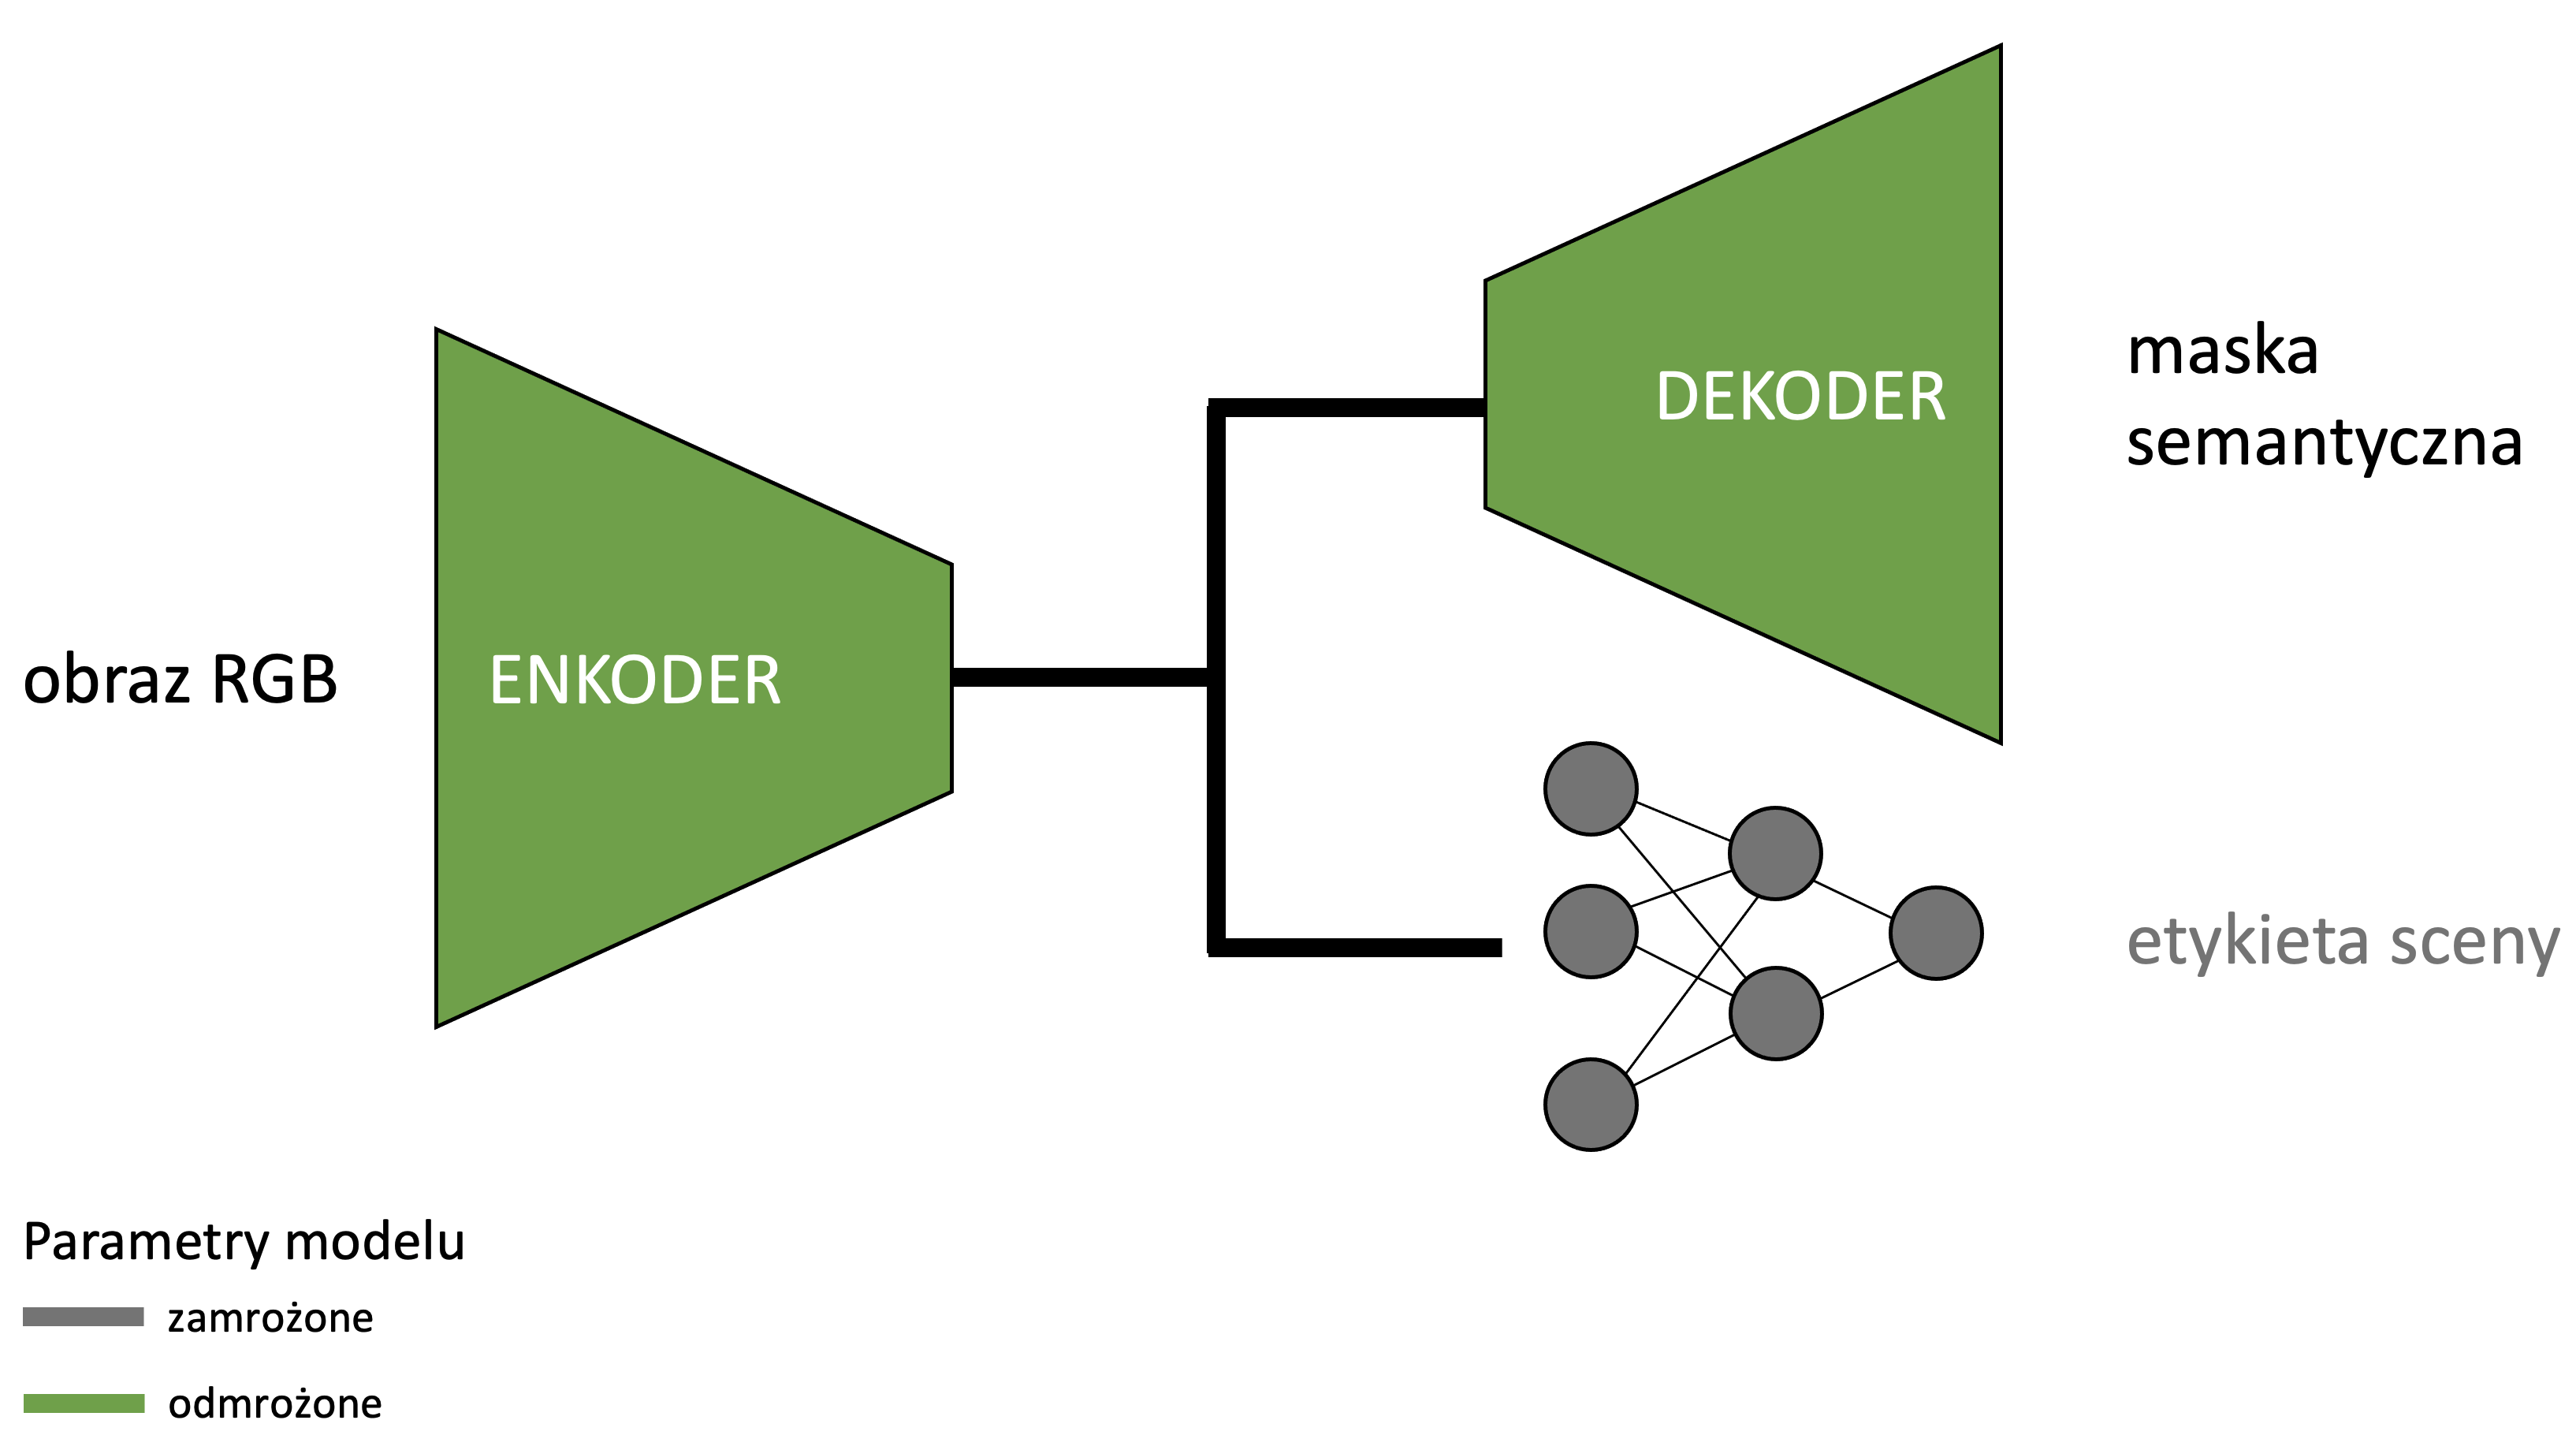
\includegraphics[width=\textwidth]{arch:seg.png}
        \caption{Architektura sieci wyłącznie w zadaniu segmentacji semantycznej.}
    \end{subfigure}
    \caption[]{Podejście jednozadaniowe.}
    \label{fig:arch-scene-seg}
\end{figure}

\begin{figure}[ht!]
    \centering
    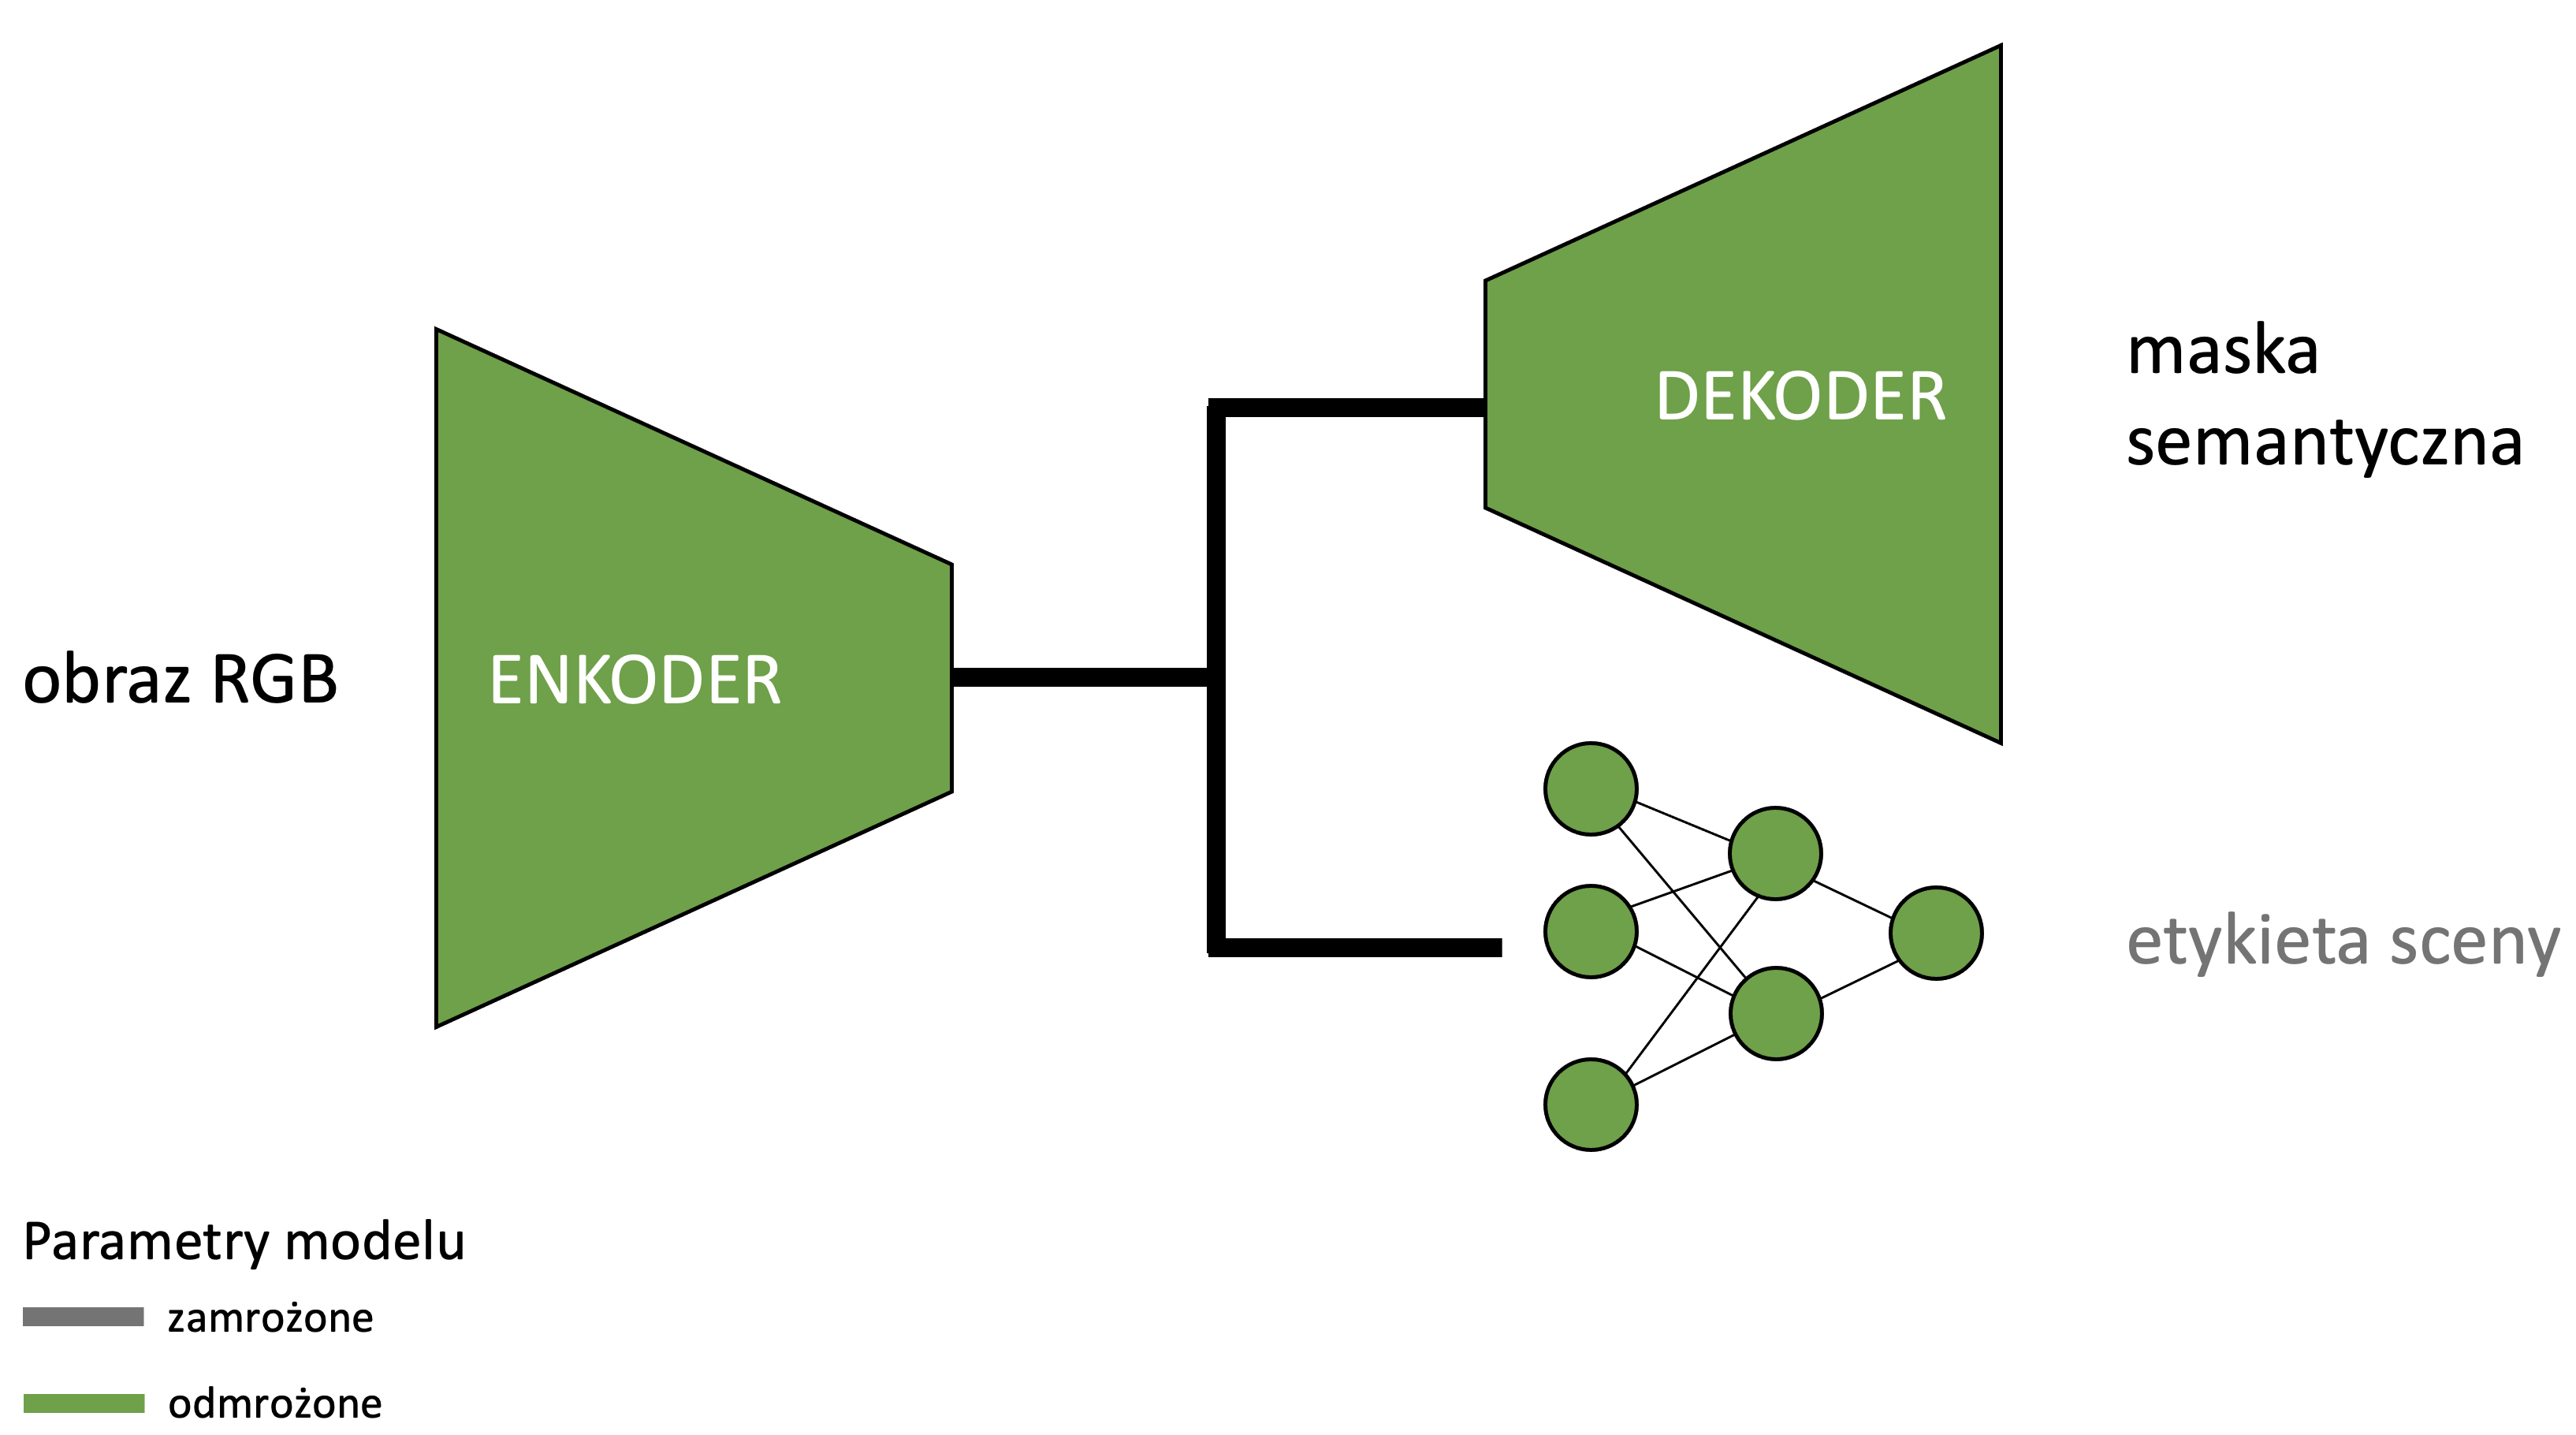
\includegraphics[width=0.75\textwidth]{arch:full.png}
    \caption{Architektura sieci jako uczenie wielozadaniowego.}
    \label{fig:arch-full}
\end{figure}